\chapter{Struktura programového řešení}
Struktura celého programového řešení je znázorněna na obrázku \ref{fig:speedy}. Celý projekt funguje následovně. Jednotlivé mikrokontroléry, resp. koncentrátory snímají potřebné veličiny, nebo čekají na impulz od uživatele sítě popř. serveru. Mohou tedy aktivně odesílat snímané informace, nebo reagovat na přijatý signál ze serveru. Tyto koncentrátory komunikují s real-time serverem pomocí protokolů TCP nebo UDP podle toho, jaký druh komunikace je pro daný účel potřeba. Server veškeré přijaté hodnoty ukládá do databáze a zároveň při každé příchozí akci prohlásí zařízení za aktivní. Udržuje tak neustále jeho status. Kromě toho, že server do databáze hodnoty ukládá, tak si také drží jednotlivé relace mezi koncentrátory resp. koncovými členy a odesílá data zpět. Tvoří tak jednotlivá propojení koncentrátorů, která je možné dynamicky měnit. Toto je asi největší výhoda tohoto řešení. Zároveň mají koncentrátory možnost zapisovat do databáze přímo. Je to dáno tím, že i se serverem komunikují v RESP formátu. Tato funkce není využívána, protože by bylo zapotřebí zapsat tvar databáze do každého koncentrátoru, což by bylo velmi omezující pro další rozšiřitelnost projektu. Nicméně tato možnost zde je a je možné ji využít pro rychlejší ukládání do databáze.

Na serveru dále běží webový server, který poskytuje webovou stránku, kde je možné celou síť ovládat. Každý uživatel sítě se pak může připojit pomocí svého zařízení (mobilní telefon, tablet, notebook, počítač, atd.) a síť ovládat. Je zřejmé, že je nutné umožnit pohodlné ovládání sítě, zároveň však musí být zamezena možnost změny konfigurace neautorizované osobě. Toto omezení je možné udělat na straně webové aplikace pomocí řízení uživatelských práv. Fakticky se jedná o změny relací v síti a o změnu parametrů jednotlivých koncových členů. Server se pak postará o distribuci dat v síti podle zvolené konfigurace.

%TODO převodní tabulky

\begin{figure}[H]
    \centering
	\makebox[\textwidth]{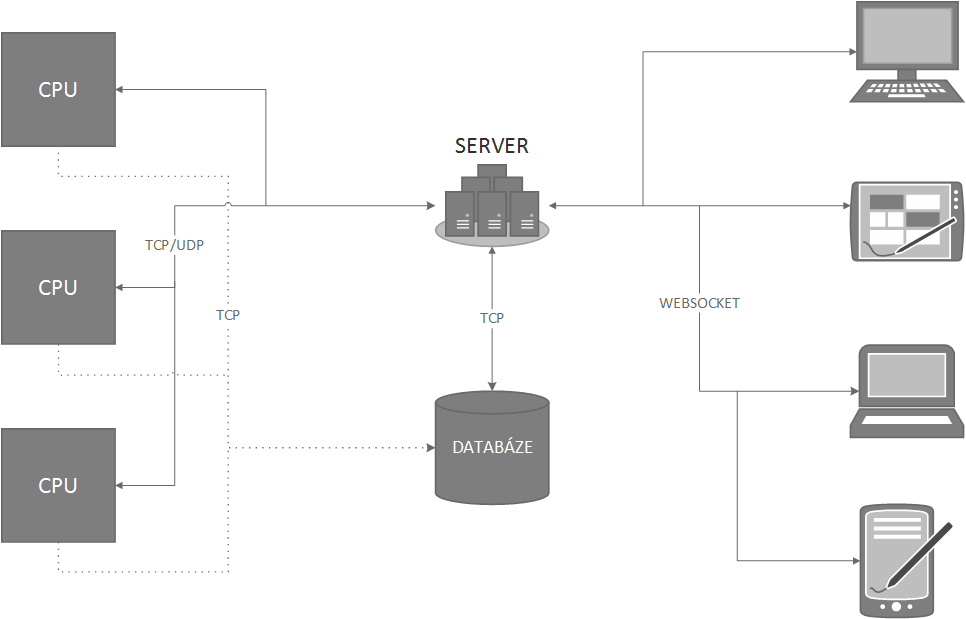
\includegraphics[width=\textwidth]{img/speedy.png}}
	\caption{Struktura programového řešení}
	\label{fig:speedy}
\end{figure}

\section{Komunikace koncentrátor - server}
Systémový firmware pro koncentrátory jsou napsány v programovacím jazyce C s využitím oficiálních Cube knihoven od STMicroelectronics. Jsou tady napsány nízkoúrovňově, ale se zachováním přijatelného programového prostředí. Koncentrátor má několik základních funkcí. Předně je jeho úkolem připojit se na pevně stanovenou IP adresu v síti. Ta je momentálně stanovena na \texttt{192.168.0.20:50000}. Koncentrátor se pak periodicky s frekvencí 1 Hz ohlašuje přes TCP serveru. Tato frekvence je zvolena libovolně s ohledem na rozumné vytížení sítě těmito jinak zbytečnými informačními pakety. Síť se tak zbytečně nevytěžuje a zároveň dochází k rychlému zaregistrování výpadku koncentrátoru. 1 Hz je navíc krajní případ, protože jakákoliv příchozí informace se zároveň považuje za ohlášení. Data jsou v RESP formátu:

\begin{minted}[breaklines]{text}
*2\r\n$4\r\nPING\r\n$11\r\nTEMP_000001\r\n
\end{minted}

První část zprávy je samotný příkaz (PING) následovaný unikátním identifikátorem zařízení. Následuje krátká vzorová ukázka funkčního kódu pro odesílání notifikací o aktivitě.

\begin{minted}[linenos,breaklines]{c}
struct tcp_pcb *client_pcb;
struct ip_addr IPaddr;

client_pcb = tcp_new();
if (client_pcb != NULL) {
  IP4_ADDR( &IPaddr, IP_ADDR0, IP_ADDR1, IP_ADDR2, IP_ADDR3 );
  tcp_bind(client_pcb, &IPaddr, DEST_PORT);
  IP4_ADDR( &DestIPaddr, DEST_IP_ADDR0, DEST_IP_ADDR1, DEST_IP_ADDR2, DEST_IP_ADDR3 );
  tcp_connect(client_pcb, &DestIPaddr, DEST_PORT, tcp_ping_callback);
} else { //can not create tcp pcb
  memp_free(MEMP_TCP_PCB, echoclient_pcb);
}
\end{minted}

Po připojení se zavolá funkce \texttt{tcp\_ping\_callback}, která již může odeslat data v požadovaném formátu.

\section{Komunikace server - koncentrátor}

\section{Komunikace server - webová aplikace}
